\chapter{КОНСТРУКТОРСКИЙ РАЗДЕЛ}\label{ch:ch2}
\section{Обоснование выбора языка программирования и среды разработки}\label{sec:ch2/sec1}
Для удобной, быстрой и эффективной, как по срокам выполнения, так и по качеству конечного продукта,
разработки {\ProgModule} потребуются правильные инструменты -- язык программирования, на котором 
легче всего описать решение данной задачи и среда разработки, не только поддерживающая данный язык,
но и позволяющая эффективно с ним работать.

\subsection{Сравнение языков программирования}\label{sec:ch2/sec1/sub1}
Для разработки {\ProgModule} понадобится сверхвысокоуровневый язык с кроссплатформенной
стандартной библиотекой, который позволит точно и лаконично описать этапы анализа,
а также имеющий высокую скорость исполнения, для анализа больших объемов исходного кода и
исполняемых файлов.
\begin{figure}[!htbp]
    \centerfloat{
        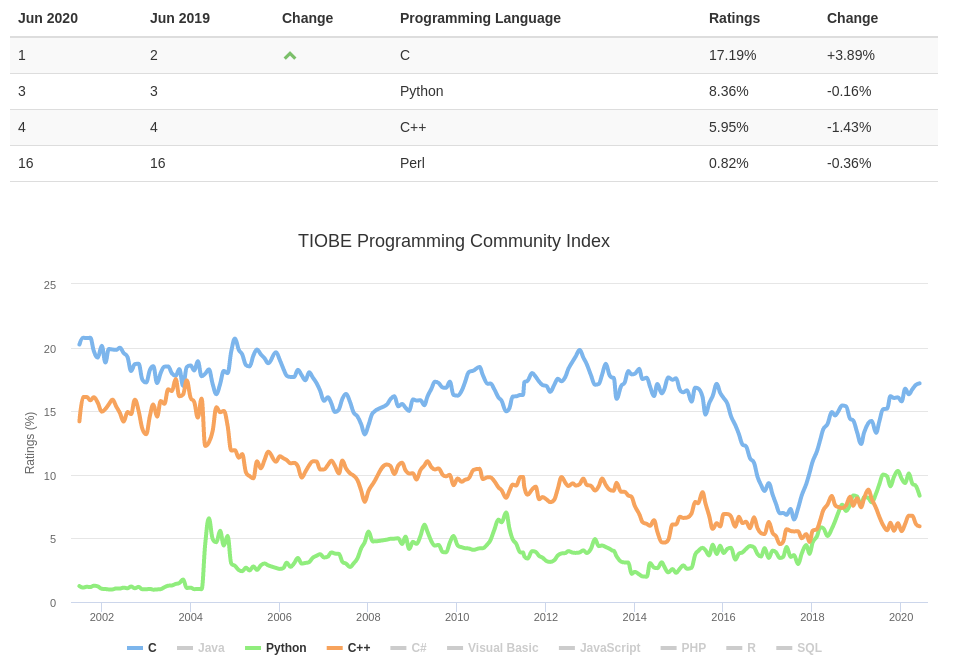
\includegraphics[width=\linewidth]{images/lang_ratings.png}
    }
    \caption{Рейтинг популярности языков программирования по версии TIOBE\label{fig:lang-ratings}}
\end{figure}

\begin{table}
    {\small
        \setlength{\tabcolsep}{2pt}
        \caption{\label{table:languages-comparsion}
               Сравнительная таблица языков программирования}
        \begin{longtable}{*{5}{| c}|}
            \hline
            \diagbox[width=8cm]{Свойства}{Язык программирования} &
                \makecell{Nim \autocite{nim}} &
                \makecell{Python \autocite{python}} &
                \makecell{Perl \autocite{perl}} &
                \makecell{C/C++} \\
            \hline
                \makecell{Сверхвысокоуровневость} & 
                \greencell{Да} & 
                \greencell{Да} &
                \greencell{Да} &
                \redcell{Нет} \\
            \hline
                \makecell{Компилируется в\\машинный код} & 
                \greencell{Да} & 
                \redcell{Нет} &
                \redcell{Нет} &
                \greencell{Да} \\
            \hline
                \makecell{Количество функции в\\стандартной библиотеке} & 
                5585 & 
                638 &
                1338 &
                1224 \\
            \hline
                \makecell{Портируемость} & 
                \greencell{Есть} & 
                \greencell{Есть} &
                \greencell{Есть} &
                \yellowcell{\makecell{Есть,\\но неудобная}}\\
            \hline
                \makecell{Встроенная\\генерация документации} & 
                \greencell{Есть} & 
                \greencell{Есть} &
                \greencell{Есть} &
                \redcell{Нет}\\
            \hline
                \makecell{Статическая типизация} & 
                \greencell{Есть} & 
                \redcell{Нет} &
                \redcell{Нет} &
                \greencell{Есть}\\
            \hline
                \makecell{Автоматическое\\управление памятью} & 
                \greencell{Есть} & 
                \greencell{Есть} &
                \greencell{Есть} &
                \greencell{Есть} \\
            \hline
                \makecell{Обобщенное программирование} & 
                \greencell{Есть} & 
                \greencell{Есть} &
                \greencell{Есть} &
                \greencell{Есть} \\
            \hline
                \makecell{Мета-программирование} & 
                \greencell{Есть} & 
                \greencell{Есть} &
                \greencell{Есть} &
                \greencell{Есть} \\
            \hline
                \makecell{Опыт использования} & 
                \greencell{Есть} & 
                \greencell{Есть} &
                \redcell{Нет} &
                \greencell{Есть} \\
            \hline
        \end{longtable}
    }
\end{table}

Рассмотрим в таблице \ref{table:languages-comparsion} подробно каждый из представленных в таблице языков.
На рисунке \ref{fig:lang-ratings} показано, как менялась популярность 
некоторых рассматриваемых языков программирования.

\subsubsection{C++}\label{sec:ch2/sec1/sub1/sub1}
Мультипарадигменный высокоуровневый язык программирования,
разработанный в 1983 году Бьёрном Страуструпом. Является практически
полным надмножеством языка C. Статически типизирован.\\
Отличается высокой производительностью и неплохой гибкостью при написании кода.
К минусам языка можно отнести сложность освоения и перегруженность 
<<наследием>> 80-х годов прошлого века, а также низкую скорость компиляции,
по сравнению с предшественником -- C.\\
Портируемость языка на различные платформы обеспечивается пере- или
кросс-компиляцией исходного кода под нужную платформу.


\subsubsection{Python}\label{sec:ch2/sec1/sub1/sub2}
Мультипарадигменный сверхвысокоуровневый язык программирования,
разработанный в 1991 году Гвидо Ван Россумом.
Является интерпретируемым языком, имеет слабую динамическую типизацию,
что позволяет легко писать обобщенный код и использовать мета-программирование,
но также ведет к трудноулавливаемым ошибкам. Негативное влияние можно сгладить
с помощью указания типов при объявлении перемнных и аргументов функций, а также 
программы, проверяющей эти типы -- линтера. Например pylint \autocite{pylint} или
pyflakes \autocite{pyflakes}.\\
Благодаря своей популярности, python также портирован на большое количество платформ.
Большим плюсом языка является его обширная стандартная библиотека, позволяющая легко
писать комплексные приложения, не прибегая к установке дополнительных библиотек --
такие программы, как и сам python, следуют философии <<в комплекте с батарейками>>
(<<batteries included>> \autocite{batteries-included}), суть которой заключается в 
самодостаточности программ. Помимо этого вместе с python поставляется менеджер
пакетов pip \autocite{pip}, позволяющий удобно устанавливать требуемые библиотечные модули вместе
с зависимостями.\\
К минусам языка можно отнести медлительность эталонного интерпретатора языка -- cpython \autocite{cpython}.
Код, исполняемый им, в определенных задачах медленнее кода на C в сотни раз. Несмотря на то, что
есть более быстрые интерпретаторы: PyPy \autocite{pypy}, Jython \autocite{jython}, Iron Python \autocite{iron-python},
они не смогут достичь скорости исполнения программ, компилируемых в машинный код.\\
На данный момент существует две, между собой несовместимые, версии языка: 
python 2, поддержка которого закончилась \DTMdate{2020-01-01}, и python 3.

\subsubsection{Perl}\label{sec:ch2/sec1/sub1/sub2}
Мультипарадигменный сверхвысокоуровневый 
язык программирования, разработанный в 1987 году Ларри Уоллом.
Является интерпретируемым языком, имеет слабую динамическую типизацию.\\
Полное название языка -- <<Practical Extraction and Report Language>> 
(<<Практический Язык для Извлечения Данных и Составления Отчётов>>), отражает его суть:
в языке реализованы обширные возможности для работы с текстом, в синтаксис интегрированы 
регулярные выражения, как и в языках, которые оказали на него наибольшее влияние --
AWK \autocite{awk} и sed \autocite{sed}. Но это же и является его слабой стороной, так как
Perl скорее предназначен для однострочных команд в терминале, как AWK и
sed.
        
\subsubsection{Nim}\label{sec:ch2/sec1/sub1/sub3}
Мультипарадигменный сверхвысокоуровневый 
язык программирования, разработанный в 2004 году Андреасом Румпфом.
Является компилируемым языком, имеет строгую статическую типизацию.

Заметно, что на синтаксис языка повлиял Python, что сделало его
выразительным и понятным. Язык использует промежуточную компиляцию, которая несколько
замедляет процесс компиляции программ, но позволяет запускать nim-программы на различных
платформах. На данный момент поддерживается компиляция в JavaScript \autocite{javascript}
и оптимизированный C-код с несколькими моделями управления памятью:\\
\begin{itemize}
    \item с автоматическими сборщиками мусора, основанные на:
        \begin{enumerate}[label={\arabic*)}]
            \item подсчете ссылок;
            \item подсчете ссылок с оптимизацией move-семантикой \autocite{nim-gc-move};
            \item boehm \autocite{boehm-gc};
            \item go \autocite{go-gc};
        \end{enumerate}
    \item ручным освобождением памяти;
    \item модель, в которой вся выделенная память высвобождается только по завершению программы
        (не рекомендуется к использованию).
\end{itemize}
Компиляция Nim в C означает не только высокую скорость работы, но и прозрачный программный интерфейс при взаимодействии с
C библиотеками. Это значит, что можно писать Nim-код, взаимодействующий с С библиотекой также, как
если бы это была Nim-библиотека, в отличие от, например, Python.\\
Так же вместе с компилятором языка поставляется пакетный менеджер nimble \autocite{nimble} и генератор
документации из комментариев, написанных на reStructuredText \autocite{restructuredtext}.

\subsubsection{Вывод}\label{sec:ch2/sec1/sub1/sub4}
Из всего вышесказанного следует, что для {\ProgModule} лучше всего подойдет язык Nim
благодаря его скорости, выразительности и портируемости на различные платформы.
Кроме того, для подготовки динамического анализа программы будут использованы утилиты, умеющие разбирать
заголовки исполняемого файла, а именно objdump и readelf. Форматирование входных данных для данных утилит
будет осуществляться с помощью Bash-скриптов. Не смотря на то, что данные программы имеются только на UNIX системах,
есть возможность использовать их и в операционной системе Windows, через Cygwin \autocite{cygwin}.

\subsection{Сравнение сред разработки}\label{sec:ch2/sec1/sub2}

Для разработки на Nim существует несколько IDE и огромное количество
текстовых редакторов, часть которых рассмотрим в таблице \ref{table:ide-comparsion}:

\begin{table}[!htbp]
    {\small
        \setlength{\tabcolsep}{2pt}
        \caption{\label{table:ide-comparsion}
               Сравнительная таблица IDE и редакторов кода}
        \begin{longtable}{*{6}{| c}|}
            \hline
            \diagbox[width=8cm]{Свойства}{IDE/Редактор} &
                \makecell{Aporia \autocite{aporia-ide}} &
                \makecell{Atom \autocite{atom-ide}} &
                \makecell{Sublime\\Text \autocite{sublime-ide}} &
                \makecell{Visual\\Studio\\Code \autocite{vs-code-ide}} &
                \makecell{Vim \autocite{vim-ide}} \\
            \hline
                \makecell{Поддержка плагинов} & 
                \redcell{Нет} &
                \greencell{Да} & 
                \greencell{Да} &
                \greencell{Да} &
                \greencell{Да} \\
            \hline
                \makecell{Требователен к ресурсам} & 
                \greencell{Нет} & 
                \redcell{Да} & 
                \greencell{Нет} & 
                \redcell{Да} & 
                \greencell{Нет} \\ 
            \hline
                \makecell{Имеет продвинутую систему\\редактирования текста} & 
                \redcell{Нет} &
                \redcell{Нет} &
                \redcell{Нет} &
                \redcell{Нет} &
                \greencell{Да} \\
            \hline
                \makecell{Кроссплатформенность} & 
                \greencell{Есть} & 
                \greencell{Есть} &
                \greencell{Есть} &
                \greencell{Есть} &
                \greencell{Есть} \\
            \hline
                \makecell{Может работать\\без GUI} & 
                \redcell{Нет} &
                \redcell{Нет} &
                \redcell{Нет} &
                \redcell{Нет} &
                \greencell{Да} \\
            \hline
                \makecell{Восстановление после сбоев} & 
                \redcell{Нет} & 
                \greencell{Есть} &
                \greencell{Есть} &
                \greencell{Есть} &
                \greencell{Есть} \\
            \hline
                \makecell{Возможность выделять\\ключевые слова с помощью\\регулярных выражений} & 
                \redcell{Нет} & 
                \greencell{Есть} &
                \greencell{Есть} &
                \greencell{Есть} &
                \greencell{Есть} \\
            \hline
                \makecell{Опыт использования} & 
                \redcell{Нет} &
                \redcell{Нет} &
                \greencell{Есть} &
                \greencell{Есть} &
                \greencell{Есть} \\
            \hline
        \end{longtable}
    }
\end{table}

Рассмотрим подробно каждый из представленных в таблице редакторов.

\subsubsection{Aporia}\label{sec:ch2/sec1/sub2/sub1}
Простая IDE, написанная на Nim, для редактирования исходного кода 
Nim, с использованием GTK2.
В настоящее время не поддерживается, так как большая часть Nim-программистов
перешла на Visual Studio Code.

\subsubsection{Atom}\label{sec:ch2/sec1/sub2/sub2}
Графический редактор с открытым исходным кодом от GitHub Inc.,
написан с использованием Electron \autocite{electron} -- фреймворка
для разработки кроссплатформенных приложений с помощью HTML, JavaScript и CSS.
Из-за архитектурных и технологических решений все программы,
написанные на данном фреймворке, являются очень требовательными
к ресурсам.

\subsubsection{Sublime Text}\label{sec:ch2/sec1/sub2/sub3}
Проприетарный графический текстовый редактор написан на C++ и python,
возможности которого могут быть расширены
с помощью плагинов на python.

\subsubsection{Visual Studio Code}\label{sec:ch2/sec1/sub2/sub4}
\begin{figure}[!htbp]
    \centerfloat{
        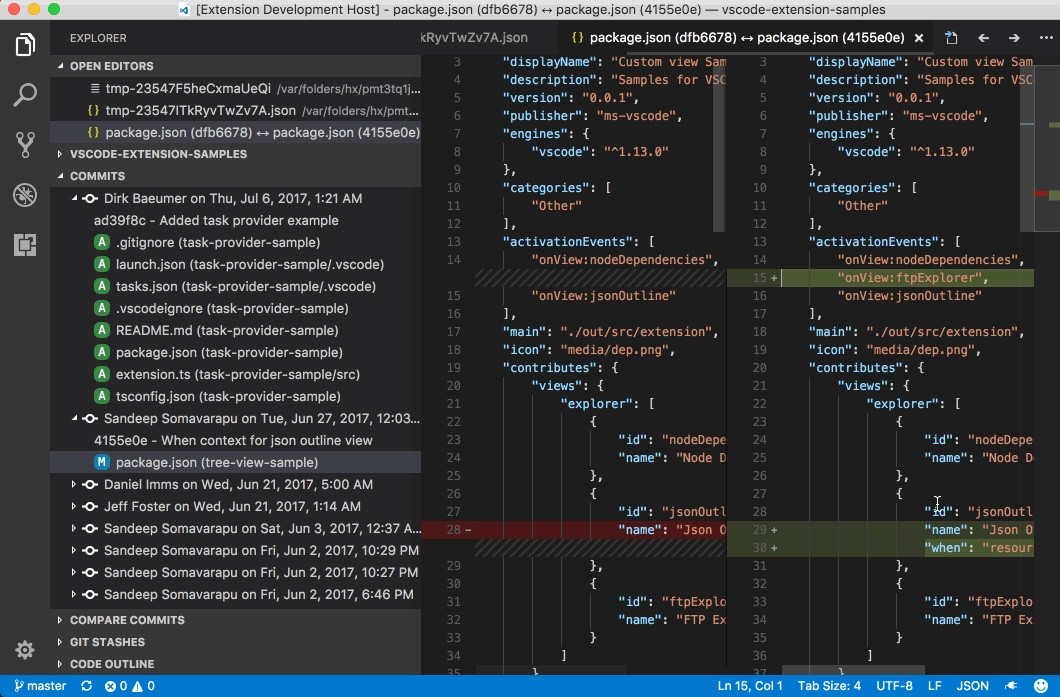
\includegraphics[width=\linewidth]{images/vscode_git.jpg}
    }
    \caption{Интеграция Git в Visual Studio Code\label{fig:vs-git}}
\end{figure}
Графический редактор с открытым исходным кодом от Microsoft.
Так же, как и Atom, написан с использованием Electron.
Имеет встроенный <<магазин>> плагинов. На текущий момент
является самым популярным редактором кода.

\subsubsection{Vim}\label{sec:ch2/sec1/sub2/sub5}
Текстовый редактор с открытым исходным кодом и большими возможностями к
быстрому редактированию текстов. Является наследником редактора vi, который, в свою
очередь, создавался с оглядкой на редактор ed. Управление делится на
режим ввода и режим команд, благодаря чему есть возможность управлять 
редактором только с помощью клавиатуры, что, при должном умении, повышает скорость
не только из-за отсутствия необходимости в использовании компьютерной мыши, но и
более коротким сочетаниям  <<горячих клавиш>>.
Поддерживает программирование необходимого функционала с помощью языка
vimscript или python. Встроенный функционал позволяет проводить сложное редактирование
в автоматическом формате, что имеет свое применение в скриптах.
Легко поддается модифицированию с помощью плагинов.
Есть под множество платформ.
\\

Так как Vim, не смотря на его расширяемость с помощью плагинов, все равно остается текстовым редактором,
то для комфортной разработки требуется дополнить его функционал возможностью компилировать, 
запускать и отлаживать {\ProgModule}. Так как Vim используется мной в качестве редактора из
консоли, для выполнения таких задач, как компиляция, отладка и запуск {\ProgModule}, то для удобной работы,
необходимо усовершенствовать именно консоль.
Для этого в систему был установлен \verb|tmux| -- терминальный мультиплексор,
позволяющий открывать в одном терминале несколько окон и удобно переключаться
между ними. Помимо этого, tmux является клиент-серверным приложением, в котором
окнами управляет tmux-сервер, а видит их tmux-клиент. Такое разделение
функционала позволяет настроить выделенный tmux-сервер, к которому можно будет
подключаться удаленно с любого устройства, поддерживающего SSH, и возвращаться,
управлять сессиями, которые были открыты с других устройств.

\subsubsection{Вывод}\label{sec:ch2/sec1/sub1/sub4}
Из всего вышесказанного и личного опыта следует, 
что для разработки {\ProgModule} лучше всего подойдет текстовый редактор Vim,
так как он поддерживает добавление плагинов, не требователен к ресурсам и позволяет
очень быстро редактировать текст. Для расширения его его функциональности использовался
терминальный мультиплексор tmux и следующие плагины:
\begin{enumerate}[label={\arabic*)}]
    \item NERDTree \autocite{nerdtree} -- улучшает просмотр каталогов;
    \item Tabular \autocite{tabular} -- позволяет быстро выравнивать текст
        для улучшения читаемости;
    \item vim-polyglot \autocite{vim-polyglot} -- подсветка синтаксиса большого
        числа языков;
    \item undotree \autocite{undotree} -- просмотр истории изменений в виде дерева;
    \item rainbow \autocite{rainbow} -- подсветка вложенных скобок разными цветами,
        для улучшения читаемости.
\end{enumerate}


\begin{figure}[!htbp]
    \centerfloat{
        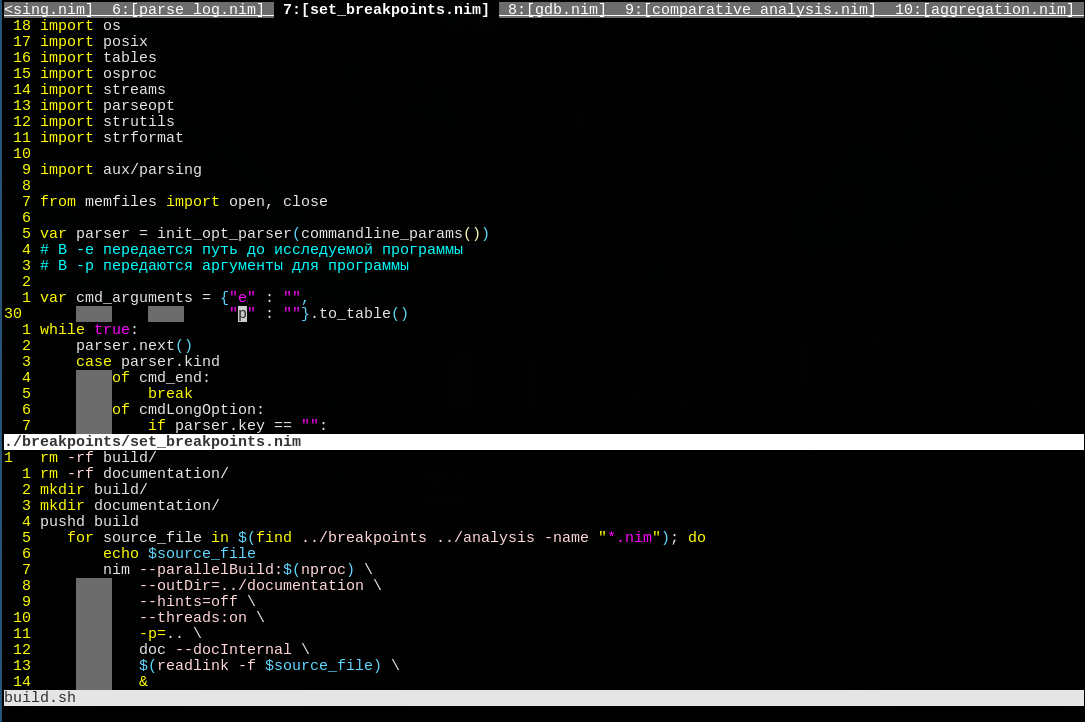
\includegraphics[width=\linewidth]{images/Vim.png}
    }
    \caption{Интерфейс Vim {\ProgModule}\label{fig:vim-tui}}
\end{figure}

\section{Архитектура {\ProgModule}}\label{sec:ch2/sec2}
Архитектура программного обеспечения объединяет внутренние
компоненты, их связи между собой и с окружением, а также принципы,
использующиеся при проектировании и эволюции программы \autocite{software-architecture}.

Поэтому было принято решение разрабатывать под каждую подзадачу проведения сертификации ПО
самостоятельную программу, которая была бы маленькой и хорошо бы справлялась со своим назначением.

При проектировании {\ProgModule} была выбрана UNIX-философия \autocite{unix-philosophy},
заключающаяся в следующих основопологающих принципах:
\begin{itemize}
    \item создавать маленькие программы;
    \item программы делают одно дело, но делают его хорошо;
    \item хранить данные в текстовом, читаемом для людей формате.
\end{itemize}

\subsection{Организация передачи информации между компонентами {\ProgModule}}\label{sec:ch2/sec2/sub1}
Передача информации между компонентами {\ProgModule} осуществляется посредством
сериализации внутренних структур (\autoref{fig:dynamic-json} и \autoref{fig:static-json})
конкретного модуля в формате JSON. JSON удобен тем, что является простым для 
чтения как человеком, так и компьютером, что позволяет оператору 
анализировать также и промежуточные результаты работы, для
вынесения вердикта.

\subsubsection{Виды сериализуемых данных}\label{sec:ch2/sec2/sub1/sub1}
В {\ProgModule} сериализуются данные после прохождения этапа:
\begin{itemize}
    \item статического анализа исходных кодов;
    \item динамического анализа сертифицируемой программы.
\end{itemize}

\begin{figure}[!htbp]
    \centerfloat{
        % !TEX encoding = UTF-8 Unicode
% Úτƒ-8 encoded
% http://www.linux.org.ru/forum/general/10357036
\tikzset{
    line/.style={draw, -latex'},
    every join/.style={line},
    u/.style={anchor=south},
    r/.style={anchor=west},
    fxd/.style={text width = 6em},
    it/.style={font={\small\itshape}},
    bf/.style={font={\small\bfseries}},
}
\tikzstyle{base} =
    [
        draw,
        on chain,
        on grid,
        align=center,
        minimum height=4ex,
        minimum width = 10ex,
        node distance = 6mm and 60mm,
        text badly centered,
    ]
\tikzstyle{coord} =
    [
        coordinate,
        on chain,
        on grid
    ]
\tikzstyle{cloud} =
    [
        base,
        ellipse,
        node distance = 3cm,
        minimum height = 2em,
        text width=2cm
    ]
\tikzstyle{decision} =
    [
        base,
        diamond,
        aspect=2,
        node distance = 2cm,
        inner sep = 0pt
    ]
\tikzstyle{block} =
    [
        rectangle,
        base,
        rounded corners,
        minimum height = 2em
    ]
\tikzstyle{print_block} =
    [
        base,
        tape,
        tape bend top=none,
    ]
\tikzstyle{io} =
    [
        base,
        trapezium,
        trapezium left angle = 70,
        trapezium right angle = 110,
    ]
\tikzstyle{prompt} =
    [
        base,
        trapezium,
        trapezium left angle = 90,
        trapezium right angle = 80,
        shape border rotate = 90
    ]
\tikzstyle{disk file} =
    [
        base,
        cylinder,
        aspect=0.2,
    ]
\tikzstyle{process} =
    [
        rectangle,
        base,
    ]
\makeatletter
\pgfkeys{/pgf/.cd,
    subrtshape w/.initial=2mm,
    cycleshape w/.initial=2mm
}
\pgfdeclareshape{parallelshape}{
    \inheritsavedanchors[from=rectangle]
    \inheritanchorborder[from=rectangle]
    \inheritanchor[from=rectangle]{north}
    \inheritanchor[from=rectangle]{center}
    \inheritanchor[from=rectangle]{west}
    \inheritanchor[from=rectangle]{east}
    \inheritanchor[from=rectangle]{mid}
    \inheritanchor[from=rectangle]{base}
    \inheritanchor[from=rectangle]{south}
    \backgroundpath{
        \southwest \pgf@xa=\pgf@x \pgf@ya=\pgf@y
        \northeast \pgf@xb=\pgf@x \pgf@yb=\pgf@y
        \def\ppd@offset{\pgfpoint{\pgfutil@tempdima}{0ex}}
        \def\ppd@offsetm{\pgfpoint{-\pgfutil@tempdima}{0ex}}
        \pgfpathmoveto{\pgfqpoint{\pgf@xa}{\pgf@ya}}
            \pgfpathlineto{\pgfqpoint{\pgf@xb}{\pgf@ya}}
        \pgfpathclose
        \pgfpathmoveto{\pgfqpoint{\pgf@xb}{\pgf@yb}}
            \pgfpathlineto{\pgfqpoint{\pgf@xa}{\pgf@yb}}
        \pgfpathclose
    }
}
\pgfdeclareshape{subrtshape}{
    \inheritsavedanchors[from=rectangle]
    \inheritanchorborder[from=rectangle]
    \inheritanchor[from=rectangle]{north}
    \inheritanchor[from=rectangle]{center}
    \inheritanchor[from=rectangle]{west}
    \inheritanchor[from=rectangle]{east}
    \inheritanchor[from=rectangle]{mid}
    \inheritanchor[from=rectangle]{base}
    \inheritanchor[from=rectangle]{south}
    \backgroundpath{
        \southwest \pgf@xa=\pgf@x \pgf@ya=\pgf@y
        \northeast \pgf@xb=\pgf@x \pgf@yb=\pgf@y
        \pgfmathsetlength\pgfutil@tempdima{\pgfkeysvalueof{/pgf/subrtshape w}}
        \def\ppd@offset{\pgfpoint{\pgfutil@tempdima}{0ex}}
        \def\ppd@offsetm{\pgfpoint{-\pgfutil@tempdima}{0ex}}
        \pgfpathmoveto{\pgfqpoint{\pgf@xa}{\pgf@ya}}
        \pgfpathlineto{\pgfqpoint{\pgf@xb}{\pgf@ya}}
        \pgfpathlineto{\pgfqpoint{\pgf@xb}{\pgf@yb}}
        \pgfpathlineto{\pgfqpoint{\pgf@xa}{\pgf@yb}}
        \pgfpathclose
        \pgfpathmoveto{\pgfpointadd{\pgfpoint{\pgf@xa}{\pgf@yb}}{\ppd@offsetm}}
        \pgfpathlineto{\pgfpointadd{\pgfpoint{\pgf@xa}{\pgf@ya}}{\ppd@offsetm}}
        \pgfpathlineto{\pgfpointadd{\pgfpoint{\pgf@xb}{\pgf@ya}}{\ppd@offset}}
        \pgfpathlineto{\pgfpointadd{\pgfpoint{\pgf@xb}{\pgf@yb}}{\ppd@offset}}
        \pgfpathclose
    }
}
\pgfdeclareshape{cyclebegshape}{
    \inheritsavedanchors[from=rectangle]
    \inheritanchorborder[from=rectangle]
    \inheritanchor[from=rectangle]{north}
    \inheritanchor[from=rectangle]{center}
    \inheritanchor[from=rectangle]{west}
    \inheritanchor[from=rectangle]{east}
    \inheritanchor[from=rectangle]{mid}
    \inheritanchor[from=rectangle]{base}
    \inheritanchor[from=rectangle]{south}
    \backgroundpath{
        \southwest \pgf@xa=\pgf@x \pgf@ya=\pgf@y
        \northeast \pgf@xb=\pgf@x \pgf@yb=\pgf@y
        \pgfmathsetlength\pgfutil@tempdima{\pgfkeysvalueof{/pgf/cycleshape w}}
        \pgfpathmoveto{\pgfqpoint{\pgf@xa}{\pgf@ya}}
\pgfpathlineto{\pgfpointadd{\pgfpoint{\pgf@xa}{\pgf@yb}}{\pgfpoint{0ex}{-\pgfutil@tempdima}}}
\pgfpathlineto{\pgfpointadd{\pgfpoint{\pgf@xa}{\pgf@yb}}{\pgfpoint{\pgfutil@tempdima}{0ex}}}
\pgfpathlineto{\pgfpointadd{\pgfpoint{\pgf@xb}{\pgf@yb}}{\pgfpoint{-\pgfutil@tempdima}{0ex}}}
\pgfpathlineto{\pgfpointadd{\pgfpoint{\pgf@xb}{\pgf@yb}}{\pgfpoint{0ex}{-\pgfutil@tempdima}}}
\pgfpathlineto{\pgfqpoint{\pgf@xb}{\pgf@ya}}
        \pgfpathclose
    }
}
\pgfdeclareshape{cycleendshape}{
    \inheritsavedanchors[from=rectangle]
    \inheritanchorborder[from=rectangle]
    \inheritanchor[from=rectangle]{north}
    \inheritanchor[from=rectangle]{center}
    \inheritanchor[from=rectangle]{west}
    \inheritanchor[from=rectangle]{east}
    \inheritanchor[from=rectangle]{mid}
    \inheritanchor[from=rectangle]{base}
    \inheritanchor[from=rectangle]{south}
    \backgroundpath{
        \southwest \pgf@xa=\pgf@x \pgf@ya=\pgf@y
        \northeast \pgf@xb=\pgf@x \pgf@yb=\pgf@y
        \pgfmathsetlength\pgfutil@tempdima{\pgfkeysvalueof{/pgf/cycleshape w}}
        \pgfpathmoveto{\pgfqpoint{\pgf@xb}{\pgf@yb}}
\pgfpathlineto{\pgfpointadd{\pgfpoint{\pgf@xb}{\pgf@ya}}{\pgfpoint{0ex}{\pgfutil@tempdima}}}
\pgfpathlineto{\pgfpointadd{\pgfpoint{\pgf@xb}{\pgf@ya}}{\pgfpoint{-\pgfutil@tempdima}{0ex}}}
\pgfpathlineto{\pgfpointadd{\pgfpoint{\pgf@xa}{\pgf@ya}}{\pgfpoint{\pgfutil@tempdima}{0ex}}}
\pgfpathlineto{\pgfpointadd{\pgfpoint{\pgf@xa}{\pgf@ya}}{\pgfpoint{0ex}{\pgfutil@tempdima}}}
\pgfpathlineto{\pgfqpoint{\pgf@xa}{\pgf@yb}}
        \pgfpathclose
    }
}
\makeatother
\tikzstyle{subroutine} =
    [
        base,
        subrtshape,
    ]
\tikzstyle{cyclebegin} =
    [
        base,
        cyclebegshape,
    ]
\tikzstyle{cycleend} =
    [
        base,
        cycleendshape,
    ]
\tikzstyle{connector} =
    [
        base,
        circle,
    ]

\tikzstyle{parallel} =
    [
        base,
        parallelshape,
    ]

\newcommand{\BreakpointInfo}{
\begin{tabular}{*{2}{| l}|}
BreakpointInfo     & Информация о точке останова\\
\hline
    address        &  адрес, на котором находится точка останова\\
    call\_address   &  адрес, по которому будет совершен вызов\\
    scope\_address  &  адрес функции, внутри которой происходит вызов\\
    registers      &  информация о регистрах процессора в момент останова\\
    instructions   &  восемь инструкций, следующих после команды вызова \\
    backtrace      &  стек вызовов\\
    stack          &  hex-dump стека программы\\
\end{tabular}
}
\newcommand{\SegmentInfo}{
\begin{tabular}{*{2}{| l}|}
SegmentInfo            & Информация о сегментах программы\\
\hline
    name               &  название сегмента\\
    occupied\_mem\_begin &  адрес памяти, с которого начинается сегмент\\
    occupied\_mem\_end   &  адрес памяти, которым заканчивается сегмент\\
\end{tabular}
}

\newcommand{\FunctionInfo}{
\begin{tabular}{*{2}{| l}|}
FunctionInfo & Информация об определенных функциях\\
\hline
    name     &  название функции\\
    address  &  адрес \\
\end{tabular}
}

\newcommand{\ProcessStartInfo}{
\begin{tabular}{*{2}{| l}|}
ProcessStartInfo & Информация о запуске исследуемой программы\\
\hline
    cmdline      &  переданные аргументы\\
    cwd          &  текущая рабочая директория\\
    exe          &  путь к исполняемому файлу\\
\end{tabular}
}

\newcommand{\ProcessSegmentsInfo}{
\begin{tabular}{*{2}{| l}|}
ProcessSegmentsInfo & Информация о всех сегментах программы\\
\hline
    entrypoint      & точка входа в программу\\
    segments        & список информации о сегментах\\
\end{tabular}
}
\newcommand{\Process}{
\begin{tabular}{*{2}{| l}|}
Process              & Информация о исследуемой программе\\
\hline
    pid              &  PID процесса\\
    start\_info       &  информация о запуске программы\\
    segments\_info    &  информация о сегментах программы\\
    breakpoints\_info &  список информации о точках останова\\
    functions\_info   &  список информации об определенных функциях\\
\end{tabular}
}

\begin{tikzpicture}[%
    start chain=going below,    % General flow is top-to-bottom
    node distance=6mm and 30mm, % Global setup of box spacing
    ] 
        \node [process] (breakpointinfo)                                          {\small \BreakpointInfo};
        \node [process] (segmentinfo)        [below = 5cm of breakpointinfo]      {\small \SegmentInfo};
        \node [process] (functioninfo)       [below = 3cm of segmentinfo]         {\small \FunctionInfo};
        \node [process] (processstartinfo)   [below = 3cm of functioninfo]        {\small \ProcessStartInfo};
        \node [process] (processsegmentsinfo)[below = 3cm of processstartinfo]    {\small \ProcessSegmentsInfo};
        \node [process] (process)            [below = 4cm of processsegmentsinfo] {\small \Process};

        \draw [line] (process) -- +(-9,-0) |- (breakpointinfo);
        \draw [line] (process) -- +(-9,-0) |- (segmentinfo);
        \draw [line] (process) -- +(-9,-0) |- (functioninfo);
        \draw [line] (process) -- +(-9,-0) |- (processstartinfo);
        \draw [line] (process) -- +(-9,-0) |- (processsegmentsinfo);

\end{tikzpicture}

    }
    \caption{Сохраняемые структуры динамического анализа \label{fig:dynamic-json}}
\end{figure}

Структура данных помогает иерархически организовать доступ к собранной, во время
динамического анализа, информации.

Данные с расставленных точек останова, содержатся в структуре \texttt{BreakpointInfo}, 
которая заполняется непосредственно во время выполнения машинных инструкций программы, а значит важно
в них получить максимальное количество информации текущем мгновенном состоянии программы.
В структуре содержится:
\begin{itemize}
    \item адреса:
            \begin{itemize}
                \item \texttt{call}-инструкции, на которой находится точка останова;
                \item по которому собирается сделать вызов \texttt{call}-инструкция;
                \item функции, в котором находится данная \texttt{call}-инструкция;
            \end{itemize}
            Которые необходимы для последующего сравнительного анализа;
        \item регистры, в которых могут содержаться передаваемые параметры (fastcall convention \autocite{fastcall});
        \item следующие за \texttt{call} 8 инструкций, в которых может содержаться код, обрабатывающий
            возвращенное значение;
        \item стек вызовов, позволяет посмотреть ветку исполнения исследуемой программы.
\end{itemize}

Информация о сегментах в \texttt{SegmentInfo} позволяет определить, к какому сегменту относится
вызываемая, или текущая функция. Например, это может быть сегмент динамически загружаемой библиотеки.

\texttt{FunctionInfo} содержит информацию, которую предоставляет GDB при загрузке программы:
список известных функций и их адреса. 

\texttt{ProcessStartInfo} сохраняет параметры запуска, \texttt{ProcessSegmentsInfo} -- 
агрегирует информацию по всем сегментам программы.
Структура \texttt{Process} же агрегирует в себе всё вышеперечисленное.

\begin{figure}[!htbp]
    \centerfloat{
        % !TEX encoding = UTF-8 Unicode
% Úτƒ-8 encoded
% http://www.linux.org.ru/forum/general/10357036
\tikzset{
    line/.style={draw, -latex'},
    every join/.style={line},
    u/.style={anchor=south},
    r/.style={anchor=west},
    fxd/.style={text width = 6em},
    it/.style={font={\small\itshape}},
    bf/.style={font={\small\bfseries}},
}
\tikzstyle{base} =
    [
        draw,
        on chain,
        on grid,
        align=center,
        minimum height=4ex,
        minimum width = 10ex,
        node distance = 6mm and 60mm,
        text badly centered,
    ]
\tikzstyle{coord} =
    [
        coordinate,
        on chain,
        on grid
    ]
\tikzstyle{cloud} =
    [
        base,
        ellipse,
        node distance = 3cm,
        minimum height = 2em,
        text width=2cm
    ]
\tikzstyle{decision} =
    [
        base,
        diamond,
        aspect=2,
        node distance = 2cm,
        inner sep = 0pt
    ]
\tikzstyle{block} =
    [
        rectangle,
        base,
        rounded corners,
        minimum height = 2em
    ]
\tikzstyle{print_block} =
    [
        base,
        tape,
        tape bend top=none,
    ]
\tikzstyle{io} =
    [
        base,
        trapezium,
        trapezium left angle = 70,
        trapezium right angle = 110,
    ]
\tikzstyle{prompt} =
    [
        base,
        trapezium,
        trapezium left angle = 90,
        trapezium right angle = 80,
        shape border rotate = 90
    ]
\tikzstyle{disk file} =
    [
        base,
        cylinder,
        aspect=0.2,
    ]
\tikzstyle{process} =
    [
        rectangle,
        base,
    ]
\makeatletter
\pgfkeys{/pgf/.cd,
    subrtshape w/.initial=2mm,
    cycleshape w/.initial=2mm
}
\pgfdeclareshape{parallelshape}{
    \inheritsavedanchors[from=rectangle]
    \inheritanchorborder[from=rectangle]
    \inheritanchor[from=rectangle]{north}
    \inheritanchor[from=rectangle]{center}
    \inheritanchor[from=rectangle]{west}
    \inheritanchor[from=rectangle]{east}
    \inheritanchor[from=rectangle]{mid}
    \inheritanchor[from=rectangle]{base}
    \inheritanchor[from=rectangle]{south}
    \backgroundpath{
        \southwest \pgf@xa=\pgf@x \pgf@ya=\pgf@y
        \northeast \pgf@xb=\pgf@x \pgf@yb=\pgf@y
        \def\ppd@offset{\pgfpoint{\pgfutil@tempdima}{0ex}}
        \def\ppd@offsetm{\pgfpoint{-\pgfutil@tempdima}{0ex}}
        \pgfpathmoveto{\pgfqpoint{\pgf@xa}{\pgf@ya}}
            \pgfpathlineto{\pgfqpoint{\pgf@xb}{\pgf@ya}}
        \pgfpathclose
        \pgfpathmoveto{\pgfqpoint{\pgf@xb}{\pgf@yb}}
            \pgfpathlineto{\pgfqpoint{\pgf@xa}{\pgf@yb}}
        \pgfpathclose
    }
}
\pgfdeclareshape{subrtshape}{
    \inheritsavedanchors[from=rectangle]
    \inheritanchorborder[from=rectangle]
    \inheritanchor[from=rectangle]{north}
    \inheritanchor[from=rectangle]{center}
    \inheritanchor[from=rectangle]{west}
    \inheritanchor[from=rectangle]{east}
    \inheritanchor[from=rectangle]{mid}
    \inheritanchor[from=rectangle]{base}
    \inheritanchor[from=rectangle]{south}
    \backgroundpath{
        \southwest \pgf@xa=\pgf@x \pgf@ya=\pgf@y
        \northeast \pgf@xb=\pgf@x \pgf@yb=\pgf@y
        \pgfmathsetlength\pgfutil@tempdima{\pgfkeysvalueof{/pgf/subrtshape w}}
        \def\ppd@offset{\pgfpoint{\pgfutil@tempdima}{0ex}}
        \def\ppd@offsetm{\pgfpoint{-\pgfutil@tempdima}{0ex}}
        \pgfpathmoveto{\pgfqpoint{\pgf@xa}{\pgf@ya}}
        \pgfpathlineto{\pgfqpoint{\pgf@xb}{\pgf@ya}}
        \pgfpathlineto{\pgfqpoint{\pgf@xb}{\pgf@yb}}
        \pgfpathlineto{\pgfqpoint{\pgf@xa}{\pgf@yb}}
        \pgfpathclose
        \pgfpathmoveto{\pgfpointadd{\pgfpoint{\pgf@xa}{\pgf@yb}}{\ppd@offsetm}}
        \pgfpathlineto{\pgfpointadd{\pgfpoint{\pgf@xa}{\pgf@ya}}{\ppd@offsetm}}
        \pgfpathlineto{\pgfpointadd{\pgfpoint{\pgf@xb}{\pgf@ya}}{\ppd@offset}}
        \pgfpathlineto{\pgfpointadd{\pgfpoint{\pgf@xb}{\pgf@yb}}{\ppd@offset}}
        \pgfpathclose
    }
}
\pgfdeclareshape{cyclebegshape}{
    \inheritsavedanchors[from=rectangle]
    \inheritanchorborder[from=rectangle]
    \inheritanchor[from=rectangle]{north}
    \inheritanchor[from=rectangle]{center}
    \inheritanchor[from=rectangle]{west}
    \inheritanchor[from=rectangle]{east}
    \inheritanchor[from=rectangle]{mid}
    \inheritanchor[from=rectangle]{base}
    \inheritanchor[from=rectangle]{south}
    \backgroundpath{
        \southwest \pgf@xa=\pgf@x \pgf@ya=\pgf@y
        \northeast \pgf@xb=\pgf@x \pgf@yb=\pgf@y
        \pgfmathsetlength\pgfutil@tempdima{\pgfkeysvalueof{/pgf/cycleshape w}}
        \pgfpathmoveto{\pgfqpoint{\pgf@xa}{\pgf@ya}}
\pgfpathlineto{\pgfpointadd{\pgfpoint{\pgf@xa}{\pgf@yb}}{\pgfpoint{0ex}{-\pgfutil@tempdima}}}
\pgfpathlineto{\pgfpointadd{\pgfpoint{\pgf@xa}{\pgf@yb}}{\pgfpoint{\pgfutil@tempdima}{0ex}}}
\pgfpathlineto{\pgfpointadd{\pgfpoint{\pgf@xb}{\pgf@yb}}{\pgfpoint{-\pgfutil@tempdima}{0ex}}}
\pgfpathlineto{\pgfpointadd{\pgfpoint{\pgf@xb}{\pgf@yb}}{\pgfpoint{0ex}{-\pgfutil@tempdima}}}
\pgfpathlineto{\pgfqpoint{\pgf@xb}{\pgf@ya}}
        \pgfpathclose
    }
}
\pgfdeclareshape{cycleendshape}{
    \inheritsavedanchors[from=rectangle]
    \inheritanchorborder[from=rectangle]
    \inheritanchor[from=rectangle]{north}
    \inheritanchor[from=rectangle]{center}
    \inheritanchor[from=rectangle]{west}
    \inheritanchor[from=rectangle]{east}
    \inheritanchor[from=rectangle]{mid}
    \inheritanchor[from=rectangle]{base}
    \inheritanchor[from=rectangle]{south}
    \backgroundpath{
        \southwest \pgf@xa=\pgf@x \pgf@ya=\pgf@y
        \northeast \pgf@xb=\pgf@x \pgf@yb=\pgf@y
        \pgfmathsetlength\pgfutil@tempdima{\pgfkeysvalueof{/pgf/cycleshape w}}
        \pgfpathmoveto{\pgfqpoint{\pgf@xb}{\pgf@yb}}
\pgfpathlineto{\pgfpointadd{\pgfpoint{\pgf@xb}{\pgf@ya}}{\pgfpoint{0ex}{\pgfutil@tempdima}}}
\pgfpathlineto{\pgfpointadd{\pgfpoint{\pgf@xb}{\pgf@ya}}{\pgfpoint{-\pgfutil@tempdima}{0ex}}}
\pgfpathlineto{\pgfpointadd{\pgfpoint{\pgf@xa}{\pgf@ya}}{\pgfpoint{\pgfutil@tempdima}{0ex}}}
\pgfpathlineto{\pgfpointadd{\pgfpoint{\pgf@xa}{\pgf@ya}}{\pgfpoint{0ex}{\pgfutil@tempdima}}}
\pgfpathlineto{\pgfqpoint{\pgf@xa}{\pgf@yb}}
        \pgfpathclose
    }
}
\makeatother
\tikzstyle{subroutine} =
    [
        base,
        subrtshape,
    ]
\tikzstyle{cyclebegin} =
    [
        base,
        cyclebegshape,
    ]
\tikzstyle{cycleend} =
    [
        base,
        cycleendshape,
    ]
\tikzstyle{connector} =
    [
        base,
        circle,
    ]

\tikzstyle{parallel} =
    [
        base,
        parallelshape,
    ]

\newcommand{\UnitInfo}{
\begin{tabular}{*{2}{| l}|}
UnitInfo & Информация об одном файле исходного кода \\
\hline
    arguments           & список аргументов компиляции \\
    directory           & папка с файлом исходного кода \\
    file                & имя файла \\
\end{tabular}
}
\newcommand{\BuildInfo}{
\begin{tabular}{*{2}{| l}|}
BuildInfo  & Информация о сборке программы \\
\hline
        units\_info          & список файлов исходного кода \\
\end{tabular}
}

\newcommand{\FunctionInfo}{
\begin{tabular}{*{2}{| l}|}
    CflowConstruct & Описание функции в статическом анализе \\
\hline
        name         & имя функции \\
        nesting      & уровень вложенности \\
        signature    & сигнатура функции \\
        path         & путь до файла, в котором используется функция \\
        line         & номер строки \\
        recursive    & рекурсивность функции \\
        text\_offset & отступ в сегменте .text \\
\end{tabular}
}

\begin{tikzpicture}[%
    start chain=going below,    % General flow is top-to-bottom
    node distance=6mm and 30mm, % Global setup of box spacing
    ] 
        \node [process] (unitinfo)                                {\small \UnitInfo};
        \node [process] (buildinfo)    [below = 4cm of unitinfo]  {\small \BuildInfo};
        \node [process] (functioninfo) [below = 4cm of buildinfo] {\small \FunctionInfo};


\end{tikzpicture}

    }
    \caption{Сохраняемые структуры статического анализа \label{fig:static-json}}
\end{figure}

Структуры данных, относящиеся к статическому анализу косвенно связаны друг с
другом. 
Их можно разделить на структуры времени компиляции программы и структуры времени статического анализа.
К структурам времени компиляции относятся:
\begin{itemize}
    \item \texttt{UnitInfo} содержит информацию о сборке одного файла исходного кода;
        В нее входит:
        \begin{itemize}
            \item аргументы компилятору -- указание заголовочных файлов, параметры генерации машинного кода,
                указание макросов и т.д.;
            \item папка, в котрой находится файл исходного кода;
            \item название файла.
        \end{itemize}
    \item \texttt{BuildInfo} агрегирует все \texttt{UnitInfo}, полученные при компиляции проекта и записанные в
        compilation database \autocite{compile-db};
\end{itemize}
К структурам времени анализа относится \texttt{CflowConstruct}, которая содержит в себе уже разобранную
и типизированную информацию, предоставляемую Cflow -- программой статического анализа:
\begin{itemize}
    \item имя функции;
    \item уровень вложенности вызова -- уровень дерева, на котором располагается конкретная функция, относительно
        точки входа -- функции с нулевым уровнем вложенности;
    \item сигнатура функции, в данном случае вместе с возвращаемым типом;
    \item путь до файла, в котором функция была использована;
    \item номер строки, где функция была использована;
    \item рекурсивность функции -- значение принимающее либо <<ложь>>, либо <<истина>>, в зависимости, есть ли в
        определении функции вызов самой себя;
    \item отступ в области .text -- количество в байтах от начала .text-сегмента уже скомпилированной программы до
        начала функции.
\end{itemize}

Все значения, кроме \texttt{text\_offset}, заполняются непосредственно во время проведения статического анализа.

\texttt{text\_offset} заполняется на стадии агрегации результатов линковки и результатов статического анлиза.
Это необходимо, чтобы на стадии сравнительного анализа можно было сопоставить адреса вызываемых функций в динамическом
и статическом анализе, полагаясь на разность между началом сегмента .text и адресом функции. Как на стадии линковки, так
и в динамическом анализе для конкретной фунции он будет одинаков.


\subsection{Cхема данных}\label{sec:ch2/sec2/sub2}

\begin{figure}[!htbp]
    \centerfloat{
        % !TEX encoding = UTF-8 Unicode
% Úτƒ-8 encoded
% http://www.linux.org.ru/forum/general/10357036
\tikzset{
    line/.style={draw, -latex'},
    every join/.style={line},
    u/.style={anchor=south},
    r/.style={anchor=west},
    fxd/.style={text width = 6em},
    it/.style={font={\small\itshape}},
    bf/.style={font={\small\bfseries}}

}
\tikzstyle{base} =
    [
        draw,
        on chain,
        on grid,
        align=center,
        minimum height=4ex,
        minimum width = 10ex,
        node distance = 6mm and 60mm,
        text badly centered,
        text width=5cm
    ]
\tikzstyle{coord} =
    [
        coordinate,
        on chain,
        on grid
    ]
\tikzstyle{cloud} =
    [
        base,
        ellipse,
        node distance = 3cm,
        minimum height = 2em
    ]
\tikzstyle{decision} =
    [
        base,
        diamond,
        aspect=2,
        node distance = 2cm,
        inner sep = 0pt
    ]
\tikzstyle{block} =
    [
        rectangle,
        base,
        rounded corners,
        minimum height = 2em
    ]
\tikzstyle{print_block} =
    [
        base,
        tape,
        tape bend top=none,
    ]
\tikzstyle{io} =
    [
        base,
        trapezium,
        trapezium left angle = 70,
        trapezium right angle = 110,
    ]
\tikzstyle{prompt} =
    [
        base,
        trapezium,
        trapezium left angle = 90,
        trapezium right angle = 80,
        shape border rotate = 90
    ]
\tikzstyle{disk file} =
    [
        base,
        cylinder,
        aspect=0.2,
    ]
\tikzstyle{process} =
    [
        rectangle,
        base,
    ]
\makeatletter
\pgfkeys{/pgf/.cd,
    subrtshape w/.initial=2mm,
    cycleshape w/.initial=2mm
}
\pgfdeclareshape{subrtshape}{
    \inheritsavedanchors[from=rectangle]
    \inheritanchorborder[from=rectangle]
    \inheritanchor[from=rectangle]{north}
    \inheritanchor[from=rectangle]{center}
    \inheritanchor[from=rectangle]{west}
    \inheritanchor[from=rectangle]{east}
    \inheritanchor[from=rectangle]{mid}
    \inheritanchor[from=rectangle]{base}
    \inheritanchor[from=rectangle]{south}
    \backgroundpath{
        \southwest \pgf@xa=\pgf@x \pgf@ya=\pgf@y
        \northeast \pgf@xb=\pgf@x \pgf@yb=\pgf@y
        \pgfmathsetlength\pgfutil@tempdima{\pgfkeysvalueof{/pgf/subrtshape w}}
        \def\ppd@offset{\pgfpoint{\pgfutil@tempdima}{0ex}}
        \def\ppd@offsetm{\pgfpoint{-\pgfutil@tempdima}{0ex}}
        \pgfpathmoveto{\pgfqpoint{\pgf@xa}{\pgf@ya}}
        \pgfpathlineto{\pgfqpoint{\pgf@xb}{\pgf@ya}}
        \pgfpathlineto{\pgfqpoint{\pgf@xb}{\pgf@yb}}
        \pgfpathlineto{\pgfqpoint{\pgf@xa}{\pgf@yb}}
        \pgfpathclose
        \pgfpathmoveto{\pgfpointadd{\pgfpoint{\pgf@xa}{\pgf@yb}}{\ppd@offsetm}}
        \pgfpathlineto{\pgfpointadd{\pgfpoint{\pgf@xa}{\pgf@ya}}{\ppd@offsetm}}
        \pgfpathlineto{\pgfpointadd{\pgfpoint{\pgf@xb}{\pgf@ya}}{\ppd@offset}}
        \pgfpathlineto{\pgfpointadd{\pgfpoint{\pgf@xb}{\pgf@yb}}{\ppd@offset}}
        \pgfpathclose
    }
}
\pgfdeclareshape{cyclebegshape}{
    \inheritsavedanchors[from=rectangle]
    \inheritanchorborder[from=rectangle]
    \inheritanchor[from=rectangle]{north}
    \inheritanchor[from=rectangle]{center}
    \inheritanchor[from=rectangle]{west}
    \inheritanchor[from=rectangle]{east}
    \inheritanchor[from=rectangle]{mid}
    \inheritanchor[from=rectangle]{base}
    \inheritanchor[from=rectangle]{south}
    \backgroundpath{
        \southwest \pgf@xa=\pgf@x \pgf@ya=\pgf@y
        \northeast \pgf@xb=\pgf@x \pgf@yb=\pgf@y
        \pgfmathsetlength\pgfutil@tempdima{\pgfkeysvalueof{/pgf/cycleshape w}}
        \pgfpathmoveto{\pgfqpoint{\pgf@xa}{\pgf@ya}}
\pgfpathlineto{\pgfpointadd{\pgfpoint{\pgf@xa}{\pgf@yb}}{\pgfpoint{0ex}{-\pgfutil@tempdima}}}
\pgfpathlineto{\pgfpointadd{\pgfpoint{\pgf@xa}{\pgf@yb}}{\pgfpoint{\pgfutil@tempdima}{0ex}}}
\pgfpathlineto{\pgfpointadd{\pgfpoint{\pgf@xb}{\pgf@yb}}{\pgfpoint{-\pgfutil@tempdima}{0ex}}}
\pgfpathlineto{\pgfpointadd{\pgfpoint{\pgf@xb}{\pgf@yb}}{\pgfpoint{0ex}{-\pgfutil@tempdima}}}
\pgfpathlineto{\pgfqpoint{\pgf@xb}{\pgf@ya}}
        \pgfpathclose
    }
}
\pgfdeclareshape{cycleendshape}{
    \inheritsavedanchors[from=rectangle]
    \inheritanchorborder[from=rectangle]
    \inheritanchor[from=rectangle]{north}
    \inheritanchor[from=rectangle]{center}
    \inheritanchor[from=rectangle]{west}
    \inheritanchor[from=rectangle]{east}
    \inheritanchor[from=rectangle]{mid}
    \inheritanchor[from=rectangle]{base}
    \inheritanchor[from=rectangle]{south}
    \backgroundpath{
        \southwest \pgf@xa=\pgf@x \pgf@ya=\pgf@y
        \northeast \pgf@xb=\pgf@x \pgf@yb=\pgf@y
        \pgfmathsetlength\pgfutil@tempdima{\pgfkeysvalueof{/pgf/cycleshape w}}
        \pgfpathmoveto{\pgfqpoint{\pgf@xb}{\pgf@yb}}
\pgfpathlineto{\pgfpointadd{\pgfpoint{\pgf@xb}{\pgf@ya}}{\pgfpoint{0ex}{\pgfutil@tempdima}}}
\pgfpathlineto{\pgfpointadd{\pgfpoint{\pgf@xb}{\pgf@ya}}{\pgfpoint{-\pgfutil@tempdima}{0ex}}}
\pgfpathlineto{\pgfpointadd{\pgfpoint{\pgf@xa}{\pgf@ya}}{\pgfpoint{\pgfutil@tempdima}{0ex}}}
\pgfpathlineto{\pgfpointadd{\pgfpoint{\pgf@xa}{\pgf@ya}}{\pgfpoint{0ex}{\pgfutil@tempdima}}}
\pgfpathlineto{\pgfqpoint{\pgf@xa}{\pgf@yb}}
        \pgfpathclose
    }
}
\makeatother
\tikzstyle{subroutine} =
    [
        base,
        subrtshape,
    ]
\tikzstyle{cyclebegin} =
    [
        base,
        cyclebegshape,
    ]
\tikzstyle{cycleend} =
    [
        base,
        cycleendshape,
    ]
\tikzstyle{connector} =
    [
        base,
        circle,
    ]
\begin{tikzpicture}[%
    start chain=going below,    % General flow is top-to-bottom
    node distance=6mm and 30mm, % Global setup of box spacing
    scale=0.7, 
    every node/.style={scale=0.72}
    ] 
        \node [prompt   ] (makefile)        [left  = 2cm ]                      {\small Путь до папки с Makefile};
        \node [process  ] (builder)         [below = 2cm of makefile]           {\small Сборщик};
        \node [prompt   ] (executable)      [right = 10cm of makefile]          {\small Путь до исполняемого файла};
        \node [process  ] (breakpointer)                                        {\small Модуль бинарного анализа};
        \node [disk file] (modified exe)    [below right = 3cm of breakpointer] {\small Модифицированный исполняемый файл};
        \node [disk file] (build log)       [below right = 3cm of builder]      {\small Файл с информацией о сборке};
        \node [process  ] (static analyzer) [below = 3cm of build log]          {\small Модуль статического анализа};
        \node [disk file] (call map)        [below left = 3cm of builder]       {\small Файл с информацией о линковке};
        \node [disk file] (gdb script)      [below left = 3cm of breakpointer]  {\small Скрипт для GDB};
        \node [process  ] (gdb manager)     [below = 4cm of breakpointer]       {\small Модуль управления отладчиком};
        \node [disk file] (dyn result)      [below = 2cm of gdb manager]        {\small Результаты динамического анализа};
        \node [process  ] (dyn parser)      [below = 2cm of dyn result]         {\small Модуль преобразования результатов динамического анализа};
        \node [disk file] (dyn json)        [below = 2cm of dyn parser]         {\small Преобразованные результаты динамического анализа};
        \node [disk file] (stat result)     [below = 2cm of static analyzer]    {\small Результаты статического анализа};
        \node [process  ] (stat parser)     [below = 2cm of stat result]        {\small Модуль преобразования результатов статического анализа};
        \node [disk file] (stat json)       [below = 2cm of stat parser]        {\small Преобразованные результаты статического анализа};
        \node [process  ] (aggregator)      [below = 2cm of stat json]          {\small Модуль агрегирования результатов линковки и статического анализа};
        \node [disk file] (aggregator file) [below = 2cm of aggregator]         {\small Агрегированные результаты линковки и статического анализа};
        \node [process  ] (comparer)                                            {\small Модуль сравнительного анализа};
        \node [disk file] (summary)                                             {\small Результаты сравнительного анализа};

        \draw [line] (makefile)        -- (builder);
        \draw [line] (builder)         -| (call map);
        \draw [line] (builder)         -| (build log);

        \draw [line] (executable)      -- (breakpointer);
        \draw [line] (breakpointer)    -| (modified exe);
        \draw [line] (breakpointer)    -| (gdb script);

        \draw [line] (modified exe)    |- (gdb manager);
        \draw [line] (gdb script)      |- (gdb manager);
        \draw [line] (gdb manager)     -- (dyn result);
        \draw [line] (dyn result)      -- (dyn parser);
        \draw [line] (dyn parser)      -- (dyn json);


        \draw [line] (build log)       -- (static analyzer);
        \draw [line] (static analyzer) -- (stat result);
        \draw [line] (stat result)     -- (stat parser);
        \draw [line] (stat parser)     -- (stat json);
        \draw [line] (call map)        |- (aggregator);
        \draw [line] (stat json)       -- (aggregator);
        \draw [line] (aggregator)      -- (aggregator file);

        \draw [line] (aggregator file) -- (comparer);
        \draw [line] (dyn json)        |- (comparer);
        \draw [line] (comparer)        -- (summary);

\end{tikzpicture}

    }
    \caption{Схема данных {\ProgModule}\label{fig:dataflow}}
\end{figure}
Из схемы данных на \autoref{fig:dataflow} видно, что работу {\ProgModule} можно разбить на параллельные 
задачи.


\subsection{Алгоритм работы {\ProgModule}}\label{sec:ch2/sec2/sub3}
Работу {\ProgModule} можно разделить на функциональные этапы:
\begin{enumerate}[label={\arabic*)}]
    \item сборка анализируемой программы;
    \item статический анализ результатов сборки\label{statical-analysis-stage};
    \item динамический анализ собранной программы\label{dynamical-analysis-stage};
    \item сравнительный анализ результатов статического и динамического анализа.
\end{enumerate}

Причем \autoref{statical-analysis-stage} и \autoref{dynamical-analysis-stage} могут выполняться
одновременно, так как не имеют зависимости по данным.

Рассмотрим подробнее каждый из этапов.

\subsubsection{Сборка анализируемой программы}\label{sec:ch2/sec2/sub3/sub1}
Этап сборки анализируемой программы в {\ProgModule} является ключевым для 
проведения статического, динамического и сравнительного анализов.
Не имеет смысла проводить анализ исполняемого файла, скомпилированного не в процессе 
проведения анализа. Без map-файла нельзя дополнить статический анализ физическими адресами
функций в исполняемом файле.
Не имея статического и динамического анализа, невозможно провести сравнительный.
При сборке программы используется утилита make и BEAR.

\paragraph{Утилита make}\label{sec:ch2/sec2/sub3/sub1/par1}\mbox{}

Make -- утилита для автоматической сборки программ и библиотек из исходного кода.
Работает через чтение специальных файлов -- <<мейкфайлов>> (англ. Makefile), в которых 
описаны <<рецепты>> сборки. В мейкфайле может находиться любое количество рецептов, они могут
быть как зависимы друг от друга, так и быть совершенно непересекающимися.

Отдельный рецепт имеет название, компоненты, от которых он зависит (могут остать пустыми, это будет означать,
что рецепт независим) и правила сборки, они тоже могут оставаться пустыми.

Стоит заметить, что использование программы make в UNIX системах не обязательно ограничевается
компиляцией программ и библиотек. В мейкфайлах с помощью рецептов также можно описать различные сценарии,
требующие последовательного выполнения команд. В большинстве программ, использующих схему распространения
через компиляцию исходного кода, имеются мейкфайлы, в которых определены рецепты clean -- очистить и help --
помощь. Которые реализуют, соответственно, очистку директорий проекта от временных файлов, полученных в результате
выполнения других рецептов мейкфайла и получения информации о доступных рецептах.

По-умолчанию, make выполняет рецепты один за другим, не начиная выполнение нового рецепта, пока
не закончится старый. Но при указании определенного аргумента, make может выполнять несвязанные рецепты
параллельно, что значительно ускоряет процесс сборки.

\paragraph{Утилита BEAR}\label{sec:ch2/sec2/sub3/sub1/par2}\mbox{}

Build EAR \autocite{bear}, или сокращенно BEAR позволяет генерировать compilation database, указывая ей
команду сборки. Compilation database или CompileDB содержит информацию о том, с какими параметрами
компилировались отдельные файлы проекта.

Сборка анализируемой программы происходит посредством программы-обертки, повторяющей интерфейс программы make
и запускающая её в контексте программы BEAR, для генерации compilation database. Помимо этого, для make
указывается генерация map-файла, файла содержащего информацию о сегментах программы,
относительных отступах функций внутри сегментов и др. После окончания компиляции дополнительно
происходит разбор сегмента .text map-файла на предмет функций и их относительных адресов внутри сегмента.
Полученные данные сохраняются на диск в JSON формате.

\subsubsection{Статический анализ результатов сборки}\label{sec:ch2/sec2/sub3/sub2}
Статический анализ результатов сборки производится с помощью программы Cflow, которой на вход
подаются аргументы компиляции, взятые из compilation database, полученной на предыдущем шаге,
а также сами файлы с исходными кодами.

Отчет Cflow состоит из списка функций, определяемых следующим правилом, описанным в \autoref{lst:cflow-rule},
где описания полей обрамлены косыми чертами:

\begin{ListingEnv}[!h]
    \captiondelim{ }
    \caption{Формат записи в отчете Cflow}\label{lst:cflow-rule}
    \begin{lstlisting}[]
{/уровень вложенности/} /имя функции/() </сигнатура функции вместе с возвращаемым значением/ at /абсолютный путь до файла/:/номер строки в файле/>:
{/уровень вложенности вызываемой функции/} /имя вызываемой функции/() </сигнатура вызываемой функции вместе с возвращаемым значением/ at /абсолютный путь до файла/:/номер строки в файле/>:

    ... 
    \end{lstlisting}
\end{ListingEnv}

Данный формат файла легко поддается разбору с помощью регулярных выражений. В {\ProgModule} использовалась
библиотека регулярных выражений PCRE \autocite{pcre}.
Не смотря на то, что Cflow умеет генерировать отчет, в которых представлен не граф вызываемых функций,
а список функций, вызывавших данную, этот формат, не смотря на удобство, страдает большим количеством
повторений, что в свою очередь вызывает слишком большой объем отчета и замедляет его разбор, из-за
чего в {\ProgModule} решено было использовать стандартную версию отчета.

\begin{ListingEnv}[!h]
    \captiondelim{ }
    \caption{Пример генерации отчета Cflow}\label{lst:cflow-example}
    \begin{Verb}[]
{   0} printsel() <void printsel (const arg *arg) at /st/st.c:1988>:
{   1}  tdumpsel() <void tdumpsel (void) at /st/st.c:1994>:
{   2}    getsel() <char *getsel (void) at /st/st.c:590>:
{   3}      xmalloc() <void *xmalloc (size_t len) at /st/st.c:253>:
{   4}        malloc()
{   4}        die() <void die (const char *errstr, ...) at /st/st.c:654>:
    \end{Verb}
\end{ListingEnv}

\subsubsection{Динамический анализ собранной программы}\label{sec:ch2/sec2/sub3/sub3}
Подготовка к динамическому анализу собранной программы начинается сразу после завершения 
этапа сборки \autoref{sec:ch2/sec2/sub3/sub1}. Путь до исполняемого файла передается в модуль расстановки
точек останова для первичного модифицирования. Модифирование заключается в том, что с помощью
программ objdump и readelf, о которых говорилось в \autoref{sec:ch2/sec1/sub1/sub4} и
небольших скриптов, написанных на bash, происходит следующее: 
\begin{enumerate}[label={\arabic*)}]
    \item находятся все \texttt{call}-инструкции, сохраняя их относительные адреса от начала сегмента .text;
    \item узнается отступ сегмента .text в байтах от начала файла;
    \item сохраняется байт по адресу, полученным на предыдущем шаге;
    \item заменяется байт по адресу, полученным на предыдущем шаге, на 0xCC в шестнадцатиричной системе счисления.
        Это машинный код инструкции \texttt{int 3} -- программного прерывания, которое используется в отладчиках
        для установки точек останова;
    \item генерируется скрипт для отладчика GDB, по расстановке точек останова на все \texttt{call}-инструкции,
        восстановлению изменений в файле и снятию состояний программы.

\end{enumerate}
Процесс исполнения данного скрипта:
\begin{enumerate}[label={\arabic*)}]
    \item \verb|file абсолютный-путь-до-файла| -- загружается исполняемый файл по абсолютному пути;
    \item выставляется формат выводимых данных:
            \begin{enumerate}[label={\arabic*)}]
                \item \verb|set disassembly-flavor intel| -- выставляется отображение синтаксиса
                    ассемблерных мнемоник в стиль intel;
                \item \verb|set input-radix 10| -- выставляется десятичная система для ввода;
                \item \verb|set args аргументы-программе| -- анализируемой программе передаются аргументы;
                \item 
                    \begin{Verbatim}
define xxd
    dump binary memory dump.bin $arg0 $arg0+$arg1
    shell xxd dump.bin >> gdb.log
end 
                    \end{Verbatim} 
                    -- определеяется команда \verb|xxd|, которая будет добавлять в лог
                            динамического анализа дамп заданного места памяти;
            \end{enumerate}
    \item \verb|run| -- запускается исследуемая программа;
    \item
        \begin{Verbatim}
info proc 
info files
info functions
        \end{Verbatim} 
        -- выводится информация о процессе, сегментах и обнаруженных функциях;
    \item программа останавливается на первом байте сегмента .text, 0xCC, кодирующем программную точку останова;
    \item \verb|set $pc--| -- счетчик команд уменьшается на единицу;
    \item \verb|set *(char*)$pc=байт| -- по адресу, указанном в счетчике команд записывается ранее сохраненный первый байт сегмента .text;
    \item расставляются относительные точки останова;
    \item программа выходит из останова и продолжает работу, собирая информацию с точек останова.
\end{enumerate}

Информация с прошедших точек останова собирается с помощью следующих команд GDB:
\begin{Verbatim}
commands
    info registers
    x/8i $pc
    bt
    xxd $sp-256 256
    continue
end
\end{Verbatim}

Нужно отметить, что в отладчике GDB существует команда \texttt{starti}, которая запускает программу и 
останавливается на первой инструкции, что позволяет отлаживать программу прямо с точки входа.
Но проблема использования \texttt{starti} состоит в том, что первой инструкцией программы может оказаться
не .text-сегмент, а какой-нибудь другой, а значит относительная расстановка точек будет неверной.
Поэтому приходится на уровне исполняемого файла удостоверяться, что исполнение программы прервется
именно на первой инструкции .text-сегмента.

\subsubsection{Сравнительный анализ результатов статического и динамического анализа}\label{sec:ch2/sec2/sub3/sub3}
Модуль сравнительного анализа запускается после того, как становятся готовы результаты статического и
динамического анализа.
Он загружает результаты с диска в описанные ранее структуры \autoref{sec:ch2/sec2/sub1/sub1}, а также
информацию о функциях из map-файла.
Это позволяет дать отчет по нескольким вариантам несовпадения:
\begin{itemize}
    \item несовпадение функций в map-файле и функций, объявленных в статическом анализе
        (каких имен из множества функций, полученных из map-файла нет среди функций, определенных в исходникых текстах);
    \item несовпадение распознанных отладчиком GDB функций и функций, полученных в динамическом анализе
        (каких имен из множества функций, определенных GDB нет среди функций, полученных из map-файла);
    \item несовпадение функций в статическом и динамическом анализе.
\end{itemize}

\begin{figure}[!htbp]
    \centerfloat{
        % !TEX encoding = UTF-8 Unicode
% Úτƒ-8 encoded
% http://www.linux.org.ru/forum/general/10357036
\tikzset{
    line/.style={draw, -latex'},
    every join/.style={line},
    u/.style={anchor=south},
    r/.style={anchor=west},
    fxd/.style={text width = 6em},
    it/.style={font={\small\itshape}},
    bf/.style={font={\small\bfseries}},
}
\tikzstyle{base_long} =
    [
        draw,
        on chain,
        on grid,
        align=center,
        minimum height=4ex,
        minimum width = 10ex,
        node distance = 6mm and 60mm,
        text badly centered,
    ]
\tikzstyle{base} =
    [
        draw,
        on chain,
        on grid,
        align=center,
        minimum height=4ex,
        minimum width = 10ex,
        node distance = 6mm and 60mm,
        text badly centered,
        text width=5cm
    ]
\tikzstyle{coord} =
    [
        coordinate,
        on chain,
        on grid
    ]
\tikzstyle{cloud} =
    [
        base,
        ellipse,
        node distance = 3cm,
        minimum height = 2em,
        text width=2cm
    ]
\tikzstyle{decision} =
    [
        base,
        diamond,
        aspect=2,
        node distance = 2cm,
        inner sep = 0pt
    ]
\tikzstyle{block} =
    [
        rectangle,
        base,
        rounded corners,
        minimum height = 2em
    ]
\tikzstyle{print_block} =
    [
        base,
        tape,
        tape bend top=none,
    ]
\tikzstyle{io} =
    [
        base,
        trapezium,
        trapezium left angle = 70,
        trapezium right angle = 110,
    ]
\tikzstyle{prompt} =
    [
        base,
        trapezium,
        trapezium left angle = 90,
        trapezium right angle = 80,
        shape border rotate = 90
    ]
\tikzstyle{disk file} =
    [
        base,
        cylinder,
        aspect=0.2,
    ]
\tikzstyle{process} =
    [
        rectangle,
        base,
    ]
\makeatletter
\pgfkeys{/pgf/.cd,
    subrtshape w/.initial=2mm,
    cycleshape w/.initial=2mm
}
\pgfdeclareshape{parallelshape}{
    \inheritsavedanchors[from=rectangle]
    \inheritanchorborder[from=rectangle]
    \inheritanchor[from=rectangle]{north}
    \inheritanchor[from=rectangle]{center}
    \inheritanchor[from=rectangle]{west}
    \inheritanchor[from=rectangle]{east}
    \inheritanchor[from=rectangle]{mid}
    \inheritanchor[from=rectangle]{base}
    \inheritanchor[from=rectangle]{south}
    \backgroundpath{
        \southwest \pgf@xa=\pgf@x \pgf@ya=\pgf@y
        \northeast \pgf@xb=\pgf@x \pgf@yb=\pgf@y
        \def\ppd@offset{\pgfpoint{\pgfutil@tempdima}{0ex}}
        \def\ppd@offsetm{\pgfpoint{-\pgfutil@tempdima}{0ex}}
        \pgfpathmoveto{\pgfqpoint{\pgf@xa}{\pgf@ya}}
            \pgfpathlineto{\pgfqpoint{\pgf@xb}{\pgf@ya}}
        \pgfpathclose
        \pgfpathmoveto{\pgfqpoint{\pgf@xb}{\pgf@yb}}
            \pgfpathlineto{\pgfqpoint{\pgf@xa}{\pgf@yb}}
        \pgfpathclose
    }
}
\pgfdeclareshape{subrtshape}{
    \inheritsavedanchors[from=rectangle]
    \inheritanchorborder[from=rectangle]
    \inheritanchor[from=rectangle]{north}
    \inheritanchor[from=rectangle]{center}
    \inheritanchor[from=rectangle]{west}
    \inheritanchor[from=rectangle]{east}
    \inheritanchor[from=rectangle]{mid}
    \inheritanchor[from=rectangle]{base}
    \inheritanchor[from=rectangle]{south}
    \backgroundpath{
        \southwest \pgf@xa=\pgf@x \pgf@ya=\pgf@y
        \northeast \pgf@xb=\pgf@x \pgf@yb=\pgf@y
        \pgfmathsetlength\pgfutil@tempdima{\pgfkeysvalueof{/pgf/subrtshape w}}
        \def\ppd@offset{\pgfpoint{\pgfutil@tempdima}{0ex}}
        \def\ppd@offsetm{\pgfpoint{-\pgfutil@tempdima}{0ex}}
        \pgfpathmoveto{\pgfqpoint{\pgf@xa}{\pgf@ya}}
        \pgfpathlineto{\pgfqpoint{\pgf@xb}{\pgf@ya}}
        \pgfpathlineto{\pgfqpoint{\pgf@xb}{\pgf@yb}}
        \pgfpathlineto{\pgfqpoint{\pgf@xa}{\pgf@yb}}
        \pgfpathclose
        \pgfpathmoveto{\pgfpointadd{\pgfpoint{\pgf@xa}{\pgf@yb}}{\ppd@offsetm}}
        \pgfpathlineto{\pgfpointadd{\pgfpoint{\pgf@xa}{\pgf@ya}}{\ppd@offsetm}}
        \pgfpathlineto{\pgfpointadd{\pgfpoint{\pgf@xb}{\pgf@ya}}{\ppd@offset}}
        \pgfpathlineto{\pgfpointadd{\pgfpoint{\pgf@xb}{\pgf@yb}}{\ppd@offset}}
        \pgfpathclose
    }
}
\pgfdeclareshape{cyclebegshape}{
    \inheritsavedanchors[from=rectangle]
    \inheritanchorborder[from=rectangle]
    \inheritanchor[from=rectangle]{north}
    \inheritanchor[from=rectangle]{center}
    \inheritanchor[from=rectangle]{west}
    \inheritanchor[from=rectangle]{east}
    \inheritanchor[from=rectangle]{mid}
    \inheritanchor[from=rectangle]{base}
    \inheritanchor[from=rectangle]{south}
    \backgroundpath{
        \southwest \pgf@xa=\pgf@x \pgf@ya=\pgf@y
        \northeast \pgf@xb=\pgf@x \pgf@yb=\pgf@y
        \pgfmathsetlength\pgfutil@tempdima{\pgfkeysvalueof{/pgf/cycleshape w}}
        \pgfpathmoveto{\pgfqpoint{\pgf@xa}{\pgf@ya}}
\pgfpathlineto{\pgfpointadd{\pgfpoint{\pgf@xa}{\pgf@yb}}{\pgfpoint{0ex}{-\pgfutil@tempdima}}}
\pgfpathlineto{\pgfpointadd{\pgfpoint{\pgf@xa}{\pgf@yb}}{\pgfpoint{\pgfutil@tempdima}{0ex}}}
\pgfpathlineto{\pgfpointadd{\pgfpoint{\pgf@xb}{\pgf@yb}}{\pgfpoint{-\pgfutil@tempdima}{0ex}}}
\pgfpathlineto{\pgfpointadd{\pgfpoint{\pgf@xb}{\pgf@yb}}{\pgfpoint{0ex}{-\pgfutil@tempdima}}}
\pgfpathlineto{\pgfqpoint{\pgf@xb}{\pgf@ya}}
        \pgfpathclose
    }
}
\pgfdeclareshape{cycleendshape}{
    \inheritsavedanchors[from=rectangle]
    \inheritanchorborder[from=rectangle]
    \inheritanchor[from=rectangle]{north}
    \inheritanchor[from=rectangle]{center}
    \inheritanchor[from=rectangle]{west}
    \inheritanchor[from=rectangle]{east}
    \inheritanchor[from=rectangle]{mid}
    \inheritanchor[from=rectangle]{base}
    \inheritanchor[from=rectangle]{south}
    \backgroundpath{
        \southwest \pgf@xa=\pgf@x \pgf@ya=\pgf@y
        \northeast \pgf@xb=\pgf@x \pgf@yb=\pgf@y
        \pgfmathsetlength\pgfutil@tempdima{\pgfkeysvalueof{/pgf/cycleshape w}}
        \pgfpathmoveto{\pgfqpoint{\pgf@xb}{\pgf@yb}}
\pgfpathlineto{\pgfpointadd{\pgfpoint{\pgf@xb}{\pgf@ya}}{\pgfpoint{0ex}{\pgfutil@tempdima}}}
\pgfpathlineto{\pgfpointadd{\pgfpoint{\pgf@xb}{\pgf@ya}}{\pgfpoint{-\pgfutil@tempdima}{0ex}}}
\pgfpathlineto{\pgfpointadd{\pgfpoint{\pgf@xa}{\pgf@ya}}{\pgfpoint{\pgfutil@tempdima}{0ex}}}
\pgfpathlineto{\pgfpointadd{\pgfpoint{\pgf@xa}{\pgf@ya}}{\pgfpoint{0ex}{\pgfutil@tempdima}}}
\pgfpathlineto{\pgfqpoint{\pgf@xa}{\pgf@yb}}
        \pgfpathclose
    }
}
\makeatother
\tikzstyle{subroutine} =
    [
        base,
        subrtshape,
    ]
\tikzstyle{cyclebegin} =
    [
        base,
        cyclebegshape,
    ]
\tikzstyle{cycleend} =
    [
        base,
        cycleendshape,
    ]
\tikzstyle{connector} =
    [
        base,
        circle,
    ]

\tikzstyle{parallel} =
    [
        base_long,
        parallelshape,
    ]
\begin{tikzpicture}[%
    start chain=going below,    % General flow is top-to-bottom
    node distance=6mm and 30mm, % Global setup of box spacing
    ] 
        \node [cloud    ] (makefile)        [left  = 4cm ]                   {\small Начало};
        \node [process  ] (builder)         [below = 3cm of makefile]        {\small Сборщик};
        \node [parallel ] (parallel)        [below of = builder, yscale=0.3] {\rptf[75]{\ }};
        \node [process  ] (breakpointer)    [below right = 5cm of builder]   {\small Бинарный анализ};
        \node [process  ] (static analyzer) [below left = 5cm of builder]    {\small Статический анализ};
        \node [process  ] (stat parser)     [below = 4cm of static analyzer] {\small Преобразование результатов статического анализа};
        \node [process  ] (aggregator)      [below = 4cm of stat parser]     {\small Агрегирование результатов линковки и статического анализа};
        \node [process  ] (gdb manager)     [below = 4cm of breakpointer]    {\small Динамический анализ};
        \node [process  ] (dyn parser)      [below = 4cm of gdb manager]     {\small Преобразование результатов динамического анализа};
        \node [cloud    ] (end)             [below = 23cm of makefile]       {\small Конец};
        \node [process  ] (comparer)        [above = 3cm of end]             {\small Сравнительный анализ};
        \node [parallel ] (parallel aggr)   [above = 3cm of comparer, yscale=0.3] {\rpts[75]{\ }};

        \draw [line] (makefile) -- (builder);
        \draw [-] (builder)     -- (parallel);

        \draw [-] (parallel)  -- +(-3.55,-0.140) -- +(-3.55,-1.9) -- (static analyzer);
        \draw [-] (parallel)  -- +(+3.55,-0.140) -- +(+3.55,-1.9) -- (breakpointer);

        \draw [line] (static analyzer) -- (stat parser);
        \draw [line] (stat parser)     -- (aggregator);

        \draw [line] (breakpointer)    -- (gdb manager);
        \draw [line] (gdb manager)     -- (dyn parser);

        \draw [-] (aggregator) -- +(+0,-1.05) -- +(+0,-2.33) -- (parallel aggr);
        \draw [-] (dyn parser) -- +(-0,-1.09) -- +(-0,-2.33) -- (parallel aggr);
        \draw [-] (parallel aggr)    -- (comparer);
        \draw [line] (comparer)        -- (end);

\end{tikzpicture}

    }
    \caption{Алгоритм работы {\ProgModule}\label{fig:algorithm}}
\end{figure}

\subsection{Разработка консольного интерфейса {\ProgModule}}\label{sec:ch2/sec2/sub4}
Программа, поддерживающая интерфейс командной строки --
компьютерная программа, обрабатывающая аргументы, переданные ей в определенном формате. 
Консольный интерфейс не может существовать без командного интерпретатора -- другой компьютерной программы, которая
обрабатывает команды компьютеру, заданные в виде текста.
Один из самых старых видов взаимодействия человека и компьютера.
Появившись в середине 1960-х, он используется и по сей день.


Для запуска {\ProgModule} с консольным интерфейсом нужно перейти в папку с собранным {\ProgModule},
после чего использовать bash-скрипт в листинге \ref{lst:run.sh}, который
принимает следующие аргументы: 
\begin{enumerate}[label={\arabic*)}]
    \item \texttt{\$1} -- путь до папки, в которой хранится мейкфайл проекта;
    \item \texttt{\$2} -- путь до исследуемого исполняемого файла.
\end{enumerate}
Результаты сравнительного анализа выводятся на экран.

\begin{ListingEnv}[!h]
    \captiondelim{ }
    \caption{run.sh}\label{lst:run.sh}
    \small
    \begin{Verb}[]
    pushd $1
        make clean
    popd
    pushd build
        ./build -C=$1
        (./set_breakpoints -e=$2 &&
         ./gdb ;
         ./parse_log &&
         ./dynamic_analysis;) &
        (./static_analysis &&
         ./aggregation) &
         wait $(jobs -p)
        ./comparative_analysis
    popd
    \end{Verb}
\end{ListingEnv}

Если же {\ProgModule} еще не собран, то нужно воспользоваться скриптом сборки (build.sh),
приведенным в листинге \ref{lst:build.sh}:
\begin{ListingEnv}[!h]
    \captiondelim{ }
    \caption{build.sh}\label{lst:build.sh}
    \small
    \begin{Verb}[]
    rm -rf build
    mkdir build 
    pushd build
       for source_file in $(find ../breakpoints ../analysis -name "*.nim"); do
           echo $source_file
           nim --parallelBuild:$(nproc) \
               --outDir=. \
               -p=.. \
               --threads:on \
               c $(readlink -f $source_file) &
       done
       wait $(jobs -p)
    popd
    \end{Verb}
\end{ListingEnv}

\subsection{Разработка графического интерфейса {\ProgModule}}\label{sec:ch2/sec2/sub5}
GUI, или графический пользовательский интерфейс впервые был показан широкой публике еще в 1968 году,
на презентации, впоследствии названной <<The Mother of All Demos>> (или <<Мать всех демонстраций>>)\autocite{mother-of-demos}.
На ней Дуглас Энгельбарт взаимодействовал с текстовым документом посредством устройства, позднее
названного компьютерной мышью, участвовал в видео конференции и совершал другие манипуляции,
предвосхитив технологии на несколько десятков лет вперед.
Первой реально использовавшейся системой с графическим интерфейсом был компьютер Xerox Alto,
разработанный в 1973 году исследователями из центра исследований Xerox в Пало-Альто, рисунок \ref{fig:xerox-alto-gui}.

\begin{figure}[!htbp]
    \centerfloat{
        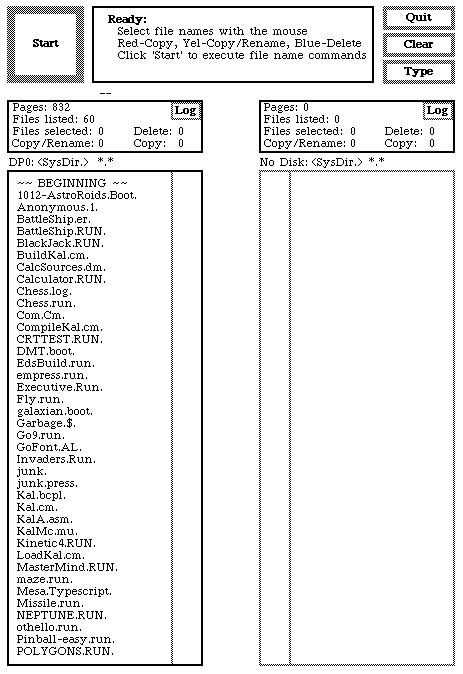
\includegraphics[scale=0.5]{images/XEROX-GUI.png}
    }
    \caption{Интерфейс файлового менеджера Xerox Alto \label{fig:xerox-alto-gui}}
\end{figure}


И сейчас, не смотря на удобстово консольного интерфейса как для программирования, так и для использования,
например, в <<Fire-and-forget>> задач, коей и старается сделать процесс сертификации {\ProgModule},
графический интерфейс остается важным элементом для обучения работы оператора с любым
программным обеспечением. Поэтому, для {\ProgModule} был создан графический интерфейс с помощью
библиотеки Gooey \autocite{gooey}.

\begin{figure}[!htbp]
    \centerfloat{
        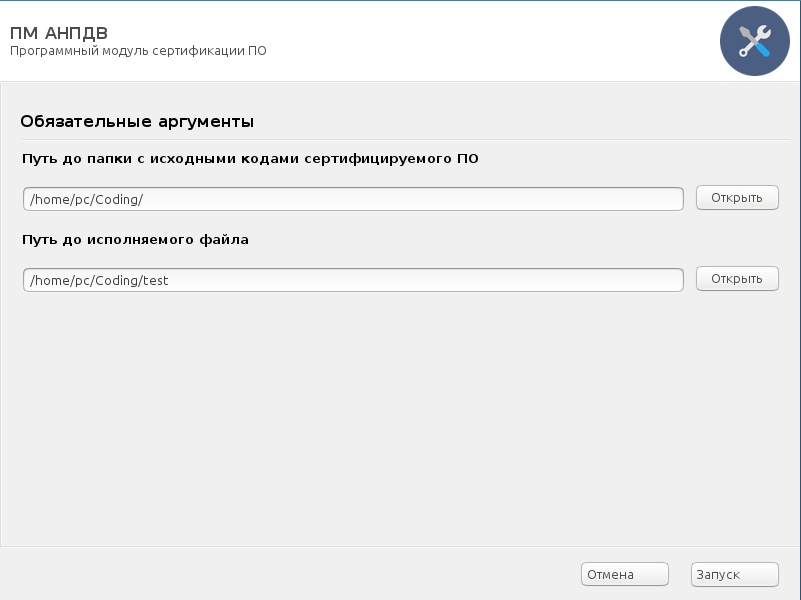
\includegraphics[trim={0.2em 0 0 0},clip,width=\linewidth]{images/apndv-gui.png}
    }
    \caption{Графический интерфейс {\ProgModule}\label{fig:apndv-gooey}}
\end{figure}

Gooey позволяет преобразовывать строку аргументов python-скрипта, созданную с помощью
модуля \verb|argparse| стандартной библиотеки в графический интерфейс, что позволяет
<<бесплатно>> добавить GUI в уже имеющуюся кодовую базу.
Помимо стандартного \verb|argparse|, Gooey предоставляет собственный парсер аргументов
командной строки, который расширяет графические возможности приложения, позволяя
использовать специфичные поля, вроде выбора даты или ввода пароля.
Так как в python удобно создавать кроссплатформенные приложения, то
данная библиотека не исключение -- внутри нее используется
обертка wxPython над библиотекой wxWidgets, что позволяет программам, использующим
Gooey быть написанными всего лишь раз и выглядеть как родные приложения той или иной
платформы.

%\begin{figure}[!htbp]
%    \centerfloat{
%        \input{images/gooey.tikz}
%    }
%    \caption{Схема работы GUI {\ProgModule}\label{fig:dynamic-json}}
%\end{figure}

\section*{Выводы по разделу}\label{sec:ch1/sec5}
\addcontentsline{toc}{section}{Выводы по разделу}
В конструкторском разделе было проведено сравнение и обоснование выбора языка программирования
и среды разработки для {\ProgModule}.
Разработана архитектура {\ProgModule}.
Также были описаны:
\begin{enumerate}[label={\arabic*)}]
    \item алгоритм передачи данных между модулями {\ProgModule};
    \item формат данных, передающихся между модулями {\ProgModule};
    \item используемые сторонние программы и форматы данных, обрабатываемые ими.
\end{enumerate}
Составлена схема данных, алгоритм работы {\ProgModule}. Описаны командный и графический интерфейс {\ProgModule}.
Подробно рассмотрены шаги выполнения процесса сертификации с помощью {\ProgModule}
